\documentclass[12pt]{article}

%-------Packages---------
\usepackage{amssymb,amsfonts}
\usepackage[all,arc]{xy}
\usepackage{enumerate}
\usepackage{mathrsfs}
\usepackage[utf8]{inputenc}
\usepackage{amsfonts}
\usepackage{amsmath}
\usepackage[shortlabels]{enumitem}
\usepackage{amsthm}
\usepackage{graphicx}
\usepackage{xcolor}
\usepackage{mdframed}
\usepackage{float}
\usepackage[lmargin=1.5in, rmargin=1in, tmargin=1in, bmargin=1in]{geometry}
\usepackage{subfigure}
\usepackage{newtxtext}

%%% hyperref stuff is taken from AGT style file
\usepackage{hyperref}  
\hypersetup{%
  bookmarksnumbered=true,%
  bookmarks=true,%
  colorlinks=true,%
  linkcolor=blue,%
  citecolor=blue,%
  filecolor=blue,%
  menucolor=blue,%
  pagecolor=blue,%
  urlcolor=blue,%
  pdfnewwindow=true,%
  pdfstartview=FitBH}   
\newcommand{\R}{\mathbb{R}}
\newcommand{\N}{\mathbb{N}}
\newcommand{\Z}{\mathbb{Z}}
\newcommand{\Q}{\mathbb{Q}}
\newcommand{\C}{\mathbb{C}}
\newcommand{\ep}{\varepsilon}
\newcommand{\LIM}{\mathop{\textup{LIM}}}
\let\fullref\autoref
%
%  \autoref is very crude.  It uses counters to distinguish environments
%  so that if say {lemma} uses the {theorem} counter, then autrorefs
%  which should come out Lemma X.Y in fact come out Theorem X.Y.  To
%  correct this give each its own counter eg:
%                 \newtheorem{theorem}{Theorem}[section]
%                 \newtheorem{lemma}{Lemma}[section]
%  and then equate the counters by commands like:
%                 \makeatletter
%                   \let\c@lemma\c@theorem
%                  \makeatother
%
%  To work correctly the environment name must have a corrresponding 
%  \XXXautorefname defined.  The following command does the job:
%
\def\makeautorefname#1#2{\expandafter\def\csname#1autorefname\endcsname{#2}}
%
%  Some standard autorefnames.  If the environment name for an autoref 
%  you need is not listed below, add a similar line to your TeX file:
%  
%\makeautorefname{equation}{Equation}%
\def\equationautorefname~#1\null{(#1)\null}
\makeautorefname{footnote}{footnote}%
\makeautorefname{item}{item}%
\makeautorefname{figure}{Figure}%
\makeautorefname{table}{Table}%
\makeautorefname{part}{Part}%
\makeautorefname{appendix}{Appendix}%
\makeautorefname{chapter}{Chapter}%
\makeautorefname{section}{Section}%
\makeautorefname{subsection}{Section}%
\makeautorefname{subsubsection}{Section}%
\makeautorefname{theorem}{Theorem}%
\makeautorefname{thm}{Theorem}%
\makeautorefname{sta}{Statement}%
\makeautorefname{cor}{Corollary}%
\makeautorefname{lem}{Lemma}%
\makeautorefname{prop}{Proposition}%
\makeautorefname{pro}{Property}
\makeautorefname{conj}{Conjecture}%
\makeautorefname{conj}{Convention}%
\makeautorefname{defn}{Definition}%
\makeautorefname{notn}{Notation}
\makeautorefname{notns}{Notations}
\makeautorefname{rem}{Remark}%
\makeautorefname{rems}{Remarks}%
\makeautorefname{quest}{Question}%
\makeautorefname{exmp}{Example}%
\makeautorefname{ax}{Axiom}%
\makeautorefname{claim}{Claim}%
\makeautorefname{ass}{Assumption}%
\makeautorefname{asses}{Assumptions}%
\makeautorefname{con}{Construction}%
\makeautorefname{prob}{Problem}%
\makeautorefname{warn}{Warning}%
\makeautorefname{obs}{Observation}%
\definecolor{problem}{rgb}{0.8,0.8,0.8}
\newcommand{\comp}[2]{
\vspace{0.2in}\begin{mdframed}[
  backgroundcolor=problem,
  userdefinedwidth=10cm,
  align=center,
  skipabove=\topsep,
  skipbelow=\topsep
  ]
  \emph{{#1}:\newline} {#2}
\end{mdframed}}

%
%                  *** End of hyperref stuff ***

\theoremstyle{plain}
\newtheorem{thm}{Theorem}[section]
\newtheorem{sta}{Statement}[section]
\newtheorem{cor}{Corollary}[section]
\newtheorem{prop}{Proposition}[section]
\newtheorem{lem}{Lemma}[section]
\newtheorem{prob}{Problem}[section]
\newtheorem{conj}{Conjecture}[section]

%\theoremstyle{theorem}
\newtheorem{defn}{Definition}[section]
\newtheorem{conv}{Convention}[section]
\newtheorem{ass}{Assumption}[section]
\newtheorem{asses}{Assumptions}[section]
\newtheorem{ax}{Axiom}[section]
\newtheorem{con}{Construction}[section]
\newtheorem{exmp}{Example}[section]
\newtheorem{notn}{Notation}[section]
\newtheorem{notns}{Notations}[section]
\newtheorem{pro}{Property}[section]
\newtheorem{quest}{Question}[section]
\newtheorem{rem}{Remark}[section]
\newtheorem{rems}{Remarks}[section]
\newtheorem{warn}{Warning}[section]
\newtheorem{sch}{Scholium}[section]
\newtheorem{obs}{Observation}[section]

%%%% hack to get fullref working correctly
\makeatletter
\let\c@obs=\c@thm
\let\c@cor=\c@thm
\let\c@prop=\c@thm
\let\c@lem=\c@thm
\let\c@prob=\c@thm
\let\c@con=\c@thm
\let\c@conj=\c@thm
\let\c@defn=\c@thm
\let\c@notn=\c@thm
\let\c@notns=\c@thm
\let\c@exmp=\c@thm
\let\c@ax=\c@thm
\let\c@pro=\c@thm
\let\c@ass=\c@thm
\let\c@warn=\c@thm
\let\c@rem=\c@thm
\let\c@conv=\c@thm
\let\c@sch=\c@thm
\numberwithin{equation}{section}
\makeatother



\bibliographystyle{plain}

%--------Meta Data: Fill in your info------

\begin{document}
\title{Optimal Transport and Applications}
\author{Aidan Copinga}
\begin{abstract}

In the 18th century, a problem was created about the best way to transport munitions to each barracks in France. This problem, now called optimal transportation, has shown useful in many fields of mathematics, from PDEs to image processing and machine learning.
This paper introduces the Monge-Kantorovich Problem and its dual problem. Using this, we are able to discuss existence of transport plans and maps of the Monge-Kantorovich problem. Finally, we cover the Wasserstein Space and applications with respect to gradient flows.

\end{abstract}
\maketitle
\tableofcontents

\subsection*{Acknowledgments}
\section{Formulation of Optimal Transport}
\subsection{Problem}
Start with a simple example where we have a pile of dirt, and a hole to fill completely with the dirt.
To transport the dirt from this pile to the hole, clearly, the volume of the hole and the pile must be the same. As is suggested in \cite{villani}, we normalize this mass to $1$.\newline
To model this rigorously, allow the pile to be space $X$ and the hole to be space $Y$. It's natural to define probability measures $\mu\in\mathcal{P}(X),\nu\in\mathcal{P}(Y)$ as mass is normalized to $1$.
In other words, for measurable $A\subset X$ and $B\subset Y$, $\mu(A)$ is the volume in the pile $X$ and $\nu(B)$ is the volume to be filled in hole $Y$.\newline
Now, introduce cost function $c: X\times Y \to \mathbb{R}$ such that for points $x\in X,y\in Y$, $c(x,y)$ represents how much energy is exhausted transporting point $x$ in the pile to point $y$ in the hole.\newline
We can now introduce the transportation problem.
%\comp{}{Given $n$ piles of sand and $m$ holes to be filled completely.}
\begin{defn}[Transportation Problem]\label{defn:tp}
Given measure spaces $X,Y$ with probability measures $\mu\in \mathcal{P}(X)$ and $\nu\in\mathcal{P}(Y)$ respectively on $X,Y$ and $c: X\times Y\to \mathbb{R}$. The Transportation Problem is realizing the transport plan from \autoref{fig:tran} while minimizing $c$.
\end{defn}
\begin{figure}[H]
  \center
  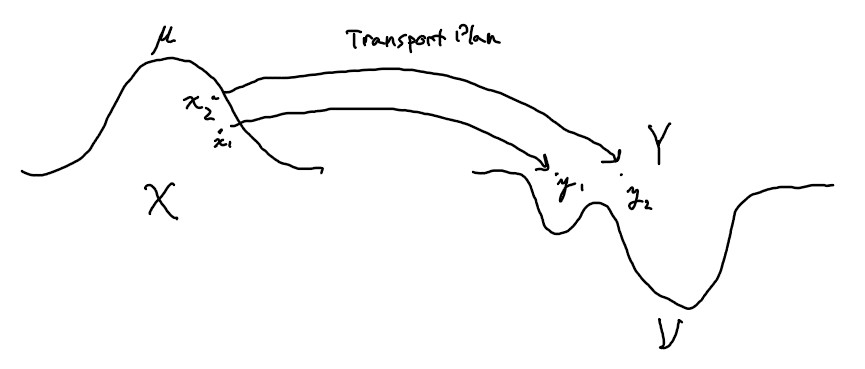
\includegraphics[scale=0.3]{transport.jpg}
  \caption{Transportation Problem}
  \label{fig:tran}
\end{figure}
There are two primary formulation for the transportation problem, the Monge and the Kantorovich formulation. The Monge formulation came historically before Kantorovich's, so I will be introducing it first.
\subsection{Monge Formulation}
\autoref{fig:tran} uses the Lagrangian framework in order to describe \autoref{defn:tp}. What this means is that particles $x\in X$ are observed individually as they are transported to $y\in Y$, and importantly, mass cannot be split, or the flows $T: X\to Y$ must be bijective.\newline From here, we introduce
the Monge formulation, which observes a transport map $T$ that transports $\mu$ to $\nu$. Before we define it, we must define what is meant by transporting one measure to another.
\begin{defn}[Transport Maps]\label{defn:transport_map}
  We say that $T: X\to Y$ transports $\mu\in \mathcal{P}(X)$ to $\nu\in\mathcal{P}(Y)$ if 
  \begin{equation*}\label{eqn:pushforward}
    \mu(T^{-1}(B)) = \nu(B) \quad\text{for all $\nu$-measurable $B\in Y$.}
  \end{equation*}
  This is typically called the \textit{pushforward} of $\mu$ and denoted as $T_\#\mu$.
\end{defn} 
In order to describe the Monge Formulation, we denote the set of all $T$ such that $T_\#\mu=\nu$ with
\begin{equation}
  \mathcal{T}(\mu,\nu) = \left\{T: X\to Y \vert T_\#\mu = \nu,\,\,\text{$T$ measurable} \right\}
\end{equation}
\begin{defn}[Monge Formulation of the transport problem]\label{defn:monge}
  \begin{equation}
    \mathbb{M}(\mu,\nu) = \underset{\mathcal{T}(\mu,\nu)}{\text{minimize}}\left\{\int_X c(x,T(x))d\mu(x)\right\}
  \end{equation}
\end{defn}
In other words, \autoref{defn:monge} is minimizing the energy required from transporting $X\overset{T(x)}{\to}Y$. 
\begin{exmp}[Discrete Monge Problem]\label{exmp:monge}
Consider $\mu = \frac{2}{3}\delta_{x_1} + \frac{1}{3}\delta_{x_2}$ and $\nu = \frac{2}{3}\delta_{y_1} + \frac{1}{3}\delta_{y_2}$. We see that the only transport map that exists is the map where $T(x_1) = y_1$ and $T(x_2)=y_2$ as such mass is not split.
However, in order to make the optimal transport map less trivial, we can allow $\mu = \frac{1}{n}\sum_{i=1}^n\delta_{x_i}$ and $\nu = \frac{1}{n}\sum_{i=1}^n\delta_{y_i}$ to create the discrete Monge optimal transportation problem. \newline
Now, we can allow $j = \sigma(i)$ where $\sigma \in S_n$ with $S_n$ be the permutations of $\{1,2\dots,n\}$. In other words, $\sigma$ is a transport map where we can define the discrete monge problem as 
\[\mathbb{M}_{\text{disc}} = \inf_{\sigma\in S_n}\left\{\frac{1}{n}\sum_{i=1}^nc(x_i,y_{\sigma(i)})\right\}.\]
\begin{figure}[H]
  \center
  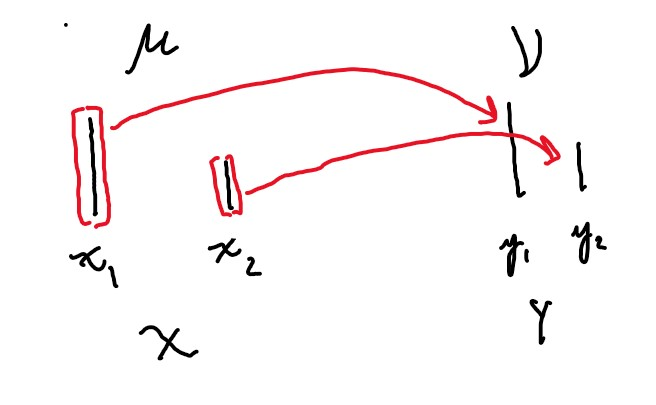
\includegraphics[scale=0.3]{monge.jpg}
  \caption{We see that $x_1\to y_1$ and $x_2\to y_2$ is the only valid transport map $T$ such that mass is not split. These are solutions to what are discrete optimal transport problems.}
  \label{fig:monge}
\end{figure}
\end{exmp}
\subsection{Kantorovich Formulation}
It's natural to ask what happens on the product space $X\times Y$. The Kantorovich does exactly this by defining \textit{transportation plans} as a product measure on $X\times Y$.

\begin{defn}[Transport Plans]
  A transport plan, $\pi \in \mathcal{P}(X\times Y)$, is valid if all mass taken from a point $x\in X$ must correspond to $d\mu(x)$ and all mass taken from a point $y\in Y$ must correspond to $d\nu(y)$, or in other terms,
  \begin{equation}\label{eqn:const}
    \pi(A\times Y) = \mu(A)\quad \pi(X\times B) = \nu(B).
  \end{equation}
\end{defn}
To define  Kantorovich's Formulation, we define the set of all probability measures that follow \autoref{eqn:const} with
\begin{equation}
  \Pi(\mu,\nu) = \left\{\pi\in \mathcal{P}(X\times Y): \text{\autoref{eqn:const} holds for all measurable $A\subset X$, $B\subset Y$}\right\}.
\end{equation}
\begin{defn}[Kantorovich Formulation of the transport problem]\label{defn:kantorovich}
  \begin{equation}
    \mathbb{K}(\mu,\nu) = \underset{\Pi(\mu,\nu)}{\text{minimize}}\left\{\int_{X\times Y} c(x,y)d\pi(x,y)\right\}.
  \end{equation}
\end{defn}
This formulation is typically referred to as a relaxation of \autoref{defn:monge}, or that Monge's problem is stronger than Kantorovich's.
\begin{prop}\label{prop:equiv}
  The Monge Formulation can be written as a Kantorovich Formulation.
\end{prop}
\begin{proof}
  Because mass cannot be split in the Monge Formulation, this means that we can rewrite $d\pi(x,y)$ in Definition \ref{defn:kantorovich}
  with
  \[ d\pi(x,y)=d\pi_T(x,y) \equiv d\mu(x)\delta[y=T(x)]\]
  where $\delta$ is the dirac measure and $T(x)$ is as defined in \autoref{defn:transport_map}. As $\int_Y\xi(x,y)\delta[y=T(x)] = \xi(x,T(x))$ for any nonnegative function $\xi:X\times Y\to \mathbb{R}$, we have that 
  \[ \int_{X\times Y}c(x,y)d\pi(x,y) = \int_X c(x,T(x))d\mu(x).\]
  In order for $\pi_T$ to be in $\Pi(\mu,\nu)$, we consider \autoref{eqn:const}
  \[\pi(A\times Y) = \mu(A)\quad \pi(X \times B) = \nu(B)\]
  so we see that this is the case where we have measurable $B\in Y$ with 
  \[\nu(B) = \mu(T^{-1}(B)).\]
  Of course, we allowed $T(x)$ to follow \autoref{defn:transport_map}, so this condition is satisfied. Furthermore, this is equivalent to the Kantorovich formulation of the transportation problem.
\end{proof}
We see that the Monge Formulation is the stronger case, where we restrict mass in $X$ from being able to be split. However, \autoref{prop:equiv} can also be framed as stating that a Kantorovich Formulation with mass
that cannot be split is a Monge Problem. Moreover, we can form a relation between the Monge and Kantorovich problem.
\begin{prop}
  $\mathbb{K}(\mu,\nu) \le \mathbb{M}(\mu,\nu)$, even if there is no optimal transport map $T_{\text{opt}}\in \mathcal{T}$
\end{prop}
\begin{proof}
  
\end{proof}
\begin{exmp}[Discrete Kantorovich Problem] Consider 
  \[\mu = \sum_{i=1}^n\alpha_i\delta_{x_i},\qquad\nu = \sum_{i=1}^n\beta_{i}\delta_{y_i}\] where $\sum_{i=1}^n \alpha_i = \sum_{i=1}^n\beta_i = 1$ and $\alpha_i \ge 0$ and $\beta_i \ge 0$. Unlike \autoref{exmp:monge}, $\alpha_i = \beta_i = \frac{1}{n}$ need not be true. Transport plans can be represented as $\pi = \pi_{ij}$\cite{thorpe} where $\pi$ is a $n\times n$ bistochastic matrix in the sense that
  \[B = \left\{\pi \bigg\vert\,\,\forall i, \quad \sum_{j=1}^n\pi_{ij} = 1;\qquad\forall j,\quad \sum_{i=1}^n\pi_{ij} = 1.\right\}\]
  So now the discrete Kantorovich problem becomes 
  \begin{equation}
    \mathbb{K}_{\text{disc}} = \inf_{\pi\in B}\sum_{i,j}\pi_{ij}c(x_i,y_j).
  \end{equation}
  \begin{figure}[H]
    \center
    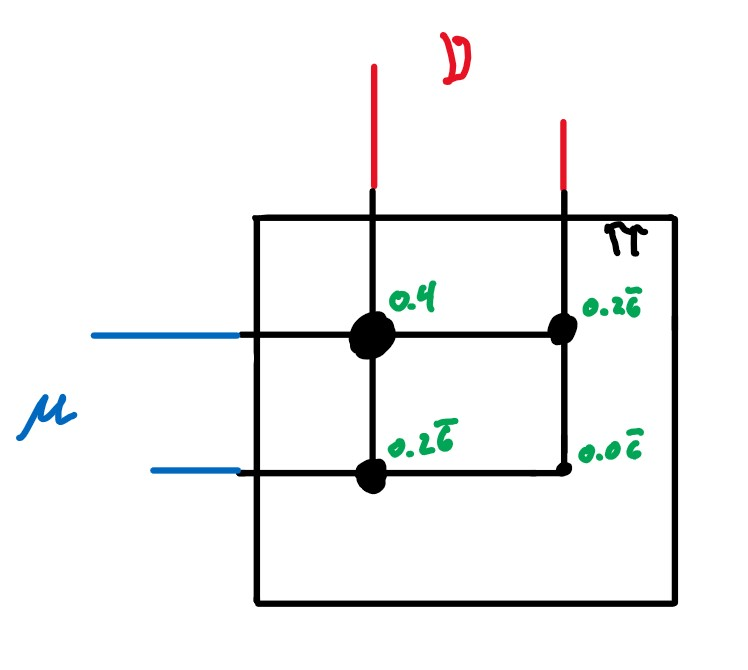
\includegraphics[scale=0.3]{discretekant.jpg}
    \caption{Letting $\mu = \frac{2}{3}\delta_{x_1} + \frac{1}{3}\delta_{x_2}$ and $\nu = \frac{2}{3}\delta_{y_1} + \frac{1}{3}\delta_{y_2}$, we see there is no concentration along the diagonal for $\pi$, hence mass is split, but this transport plan is still valid.}
    \label{fig:kant}
  \end{figure}
\end{exmp} 
\section{Existence and Characterization of Transport Plans}

\subsection{Direct Method in Calculus of Variations}
\begin{exmp}[Direct Method]
  Given a bounded domain $U\in \R^n$, consider the Dirichlet problem for the Laplace equation $\Delta u = 0$ in $U$ with $u-\phi \in H_0^1(U)$ for some $\phi \in H^1(U)$. Now set the Dirichlet energy,
  \[I[v] = \int_U |Dv|^2dx\]
  The task is to find $\min_{v\in\mathcal{A}} I[v]$ where $\mathcal{A} = \{v\in H^1(U) : v - \phi \in H^1_0(U)\}$.
\end{exmp}
\begin{proof}
  Set $m = \inf_{v\in\mathcal{A}} I[v]$, and take a minimizing sequence $\{u_k\}_{k=1}^\infty$. Because $u_k$ is a minimizing sequence, we can assume there exists $C \ge 0$ such that $I[u_k]\le C$ for all $k$. Then,
  \[\int_U |D(u_k - \phi)|^2 dx \le C + \|D\phi\|_{L^2(U)}\]
  and by Poincar\'e's inequality, we have that 
  \[\|u_k-\phi\|_{L^2(U)} \le C\|D(u_k-\phi)\|_{L^2(U)}\]
  and thus $u_k$ is bounded in $H^1(U)$. Moreover, there exists a weakly convergence subsequence 
  \(u_{k_l}\rightharpoonup u\in H^1(U)\) so both \(u_{k_l}\rightharpoonup u,\text{ and }Du_{k_l}\rightharpoonup Du\in L^1(U)\).\newline
  Because a closed convex subset of a normed space is weakly closed, the norm is weakly semicontinuous, and we can conclude that 
  \[\int_U |Du|^2 dx \le \liminf_{l\to\infty}\int_U |Du_{k_l}|^2dx = m.\]
  Moreover, because $I[u]$ is itself a minimum, it's not difficult to verify that $u$ solves the Dirichlet problem.
\end{proof}
What was used here is called the \textit{direct method}, and it's often seen in Calculus of Variations for characterizing existence of minimizers. We start by defining Lagrangians over $\R^n$ as is done in \cite{evans}.
\begin{defn}[Lagrangians]\label{defn:lagrangian}
  Let $X \subset \R^n$. A function $\mathcal{L} : (X, \R,\R^n) \to \R$ is called a Lagrangian if 
  \begin{enumerate}
    \item Coercivity - There exists $\alpha \in \R_+$ and $\beta\in \R$ such that $\mathcal{L}(x,z,p) \ge \alpha|p|^q - \beta$ for all $x\in X$, $z\in \R$, and $p\in\R^n$.
    \item Convexity in the $p$-variable - The mapping $p\mapsto \mathcal{L}(x,z,p)$ is convex for each $x\in X$,$z\in \R$. Moreover, for each $\xi\in\R^n$, $\mathcal{L}_{p_ip_j}\xi_i\xi_j \ge 0$.
  \end{enumerate}
\end{defn}
We then look at minimizing the functional 
\[I[v] = \int_{X}\mathcal{L}(x,v,Dv)dx\]
where $v : X\to\R$ over $v$ in a given class. Importantly, condition 2. of \autoref{defn:lagrangian} implies that $\mathcal{L}$ is lower semicontinuous. Recall that $W^{p,q}$ is the Sobolev space of functions that are $p$ times differentiable with derivatives in $L^q$.
\begin{thm}
  If $\mathcal{L}$ is bounded below and convex in the $p$-variable, then $I[\cdot]$ is weakly lower semicontinuous on $W^{1,q}(X).$ That is, $I[u] \le \liminf_{k\to\infty} I[u_k]$ where $u_k\rightharpoonup u$ in $W^{1,q}(X)$.
\end{thm}
Now, we can discuss minimizers in $W^{1,q}$.
\begin{thm}
  If $\mathcal{L}$ is a Lagrangian and the admissable class of functions $\mathcal{A}$ is nonempty, then $I[u] := \min_{v\in\mathcal{A}} I[v]$.\newline
  $u$ is the unique minimizer if $\mathcal{L}$ does not depend on $z$ and if there exists $\theta > 0$ such that $\sum_{i,j}\mathcal{L}_{p_ip_j}\xi_i\xi_j\ge \theta|\xi|^2$ for all $p,\xi\in\R^n$ and $x\in X$.
\end{thm}
\begin{proof}
  Theorem 8.2.2 and 8.2.3 in \cite{evans}.
\end{proof}
In general, we can define the direct method as follows.
\begin{defn}[Direct Method]\label{defn:direct}
  Given a functional $I$ and a nonempty admissable class $\mathcal{A}$. If $I$ is bounded below, then the \textit{direct method} is defined as 
  \begin{enumerate}
    \item Take a minimizing sequence $\{u_k\}\in \mathcal{A}$ for $I$.
    \item Show that there is a subsequence $\{u_{k_l}\}\in \mathcal{A}$ which converges to $u\in \mathcal{A}$ with respect to the topology on $\mathcal{A}$.
    \item Show that $I$ is lower semicontinuous with respect to the topology on $\mathcal{A}$.
  \end{enumerate}
  If all three steps are satisfied, then $u$ will be a minimizer of $\inf_{v\in\mathcal{A}} I[v]$.
\end{defn}
\subsection{Existence of Transport Plans}
Using \autoref{defn:direct}, we can discuss the existence of transport plans, or rather, the existence of optimal plans in the sense of \autoref{defn:kantorovich}. \autoref{prop:existence_plan} is taken from Proposition 2.1 in \cite{villani}. Prior to this, I will introduce Prokhorov's theorem.
\begin{thm}[Prokhorov's Theorem]
  If $(S,\rho)$ is a separable metric space, then $K\subset \mathcal{P}(S)$ is tight if and only if the closure of $K$ is sequentially compact in $\mathcal{P}(S)$ in the weak$\star$ topology.
\end{thm}
\begin{prop}\label{prop:existence_plan}
  Let $X,Y$ be polish spaces with probability measures $\mu,\nu$ respectively. If $c : X\times Y \to [0,\infty)$ is lower semi-continuous, then there exists $\gamma\in \Pi(\mu,\nu)$
  that is the optimal transport plan that solves \autoref{defn:kantorovich}. 
\end{prop}
\begin{proof}
  $\Pi(\nu,\mu)$ is nonempty as the tensor product $\mu\otimes \nu$ is in $\Pi$. Let $\delta > 0$ and compact sets $K\subset X$ and $L\subset Y$ such that 
  \[\mu(X\setminus K) \le \delta,\qquad \nu(Y\setminus L)\le \delta\]
  as $\mu,\nu$ are inner regular by definition. Now, consider $(x,y)\in (X\times Y)\setminus (K\times L)$. $x\notin K$ or $y\notin L$ so for any $\pi\in\Pi(\mu,\nu)$, 
  \begin{align*}
    \pi((X\times Y)\setminus (K\times L)) &\le \pi(X\times (Y\setminus L)) + \pi((X\setminus K)\times Y) \\
    &= \nu(Y\setminus L) + \mu(X\setminus K) \le 2\delta.
  \end{align*}
  Hence $\Pi(\mu,\nu)$ is tight. Then, by Prokhorov's theorem, $\overline{\Pi(\mu,\nu)}$ is sequentially compact in the weak$\star$ topology.\newline
  Let $\pi_n\in\Pi(\mu,\nu)$ be a sequence such that for some $\pi\in M(X\times Y)$, $\pi_n\overset{\star}{\rightharpoonup} \pi$. Fix $d\in X$ and $c\in Y$. Now let $f_1(x,c) \in C_b(X\times Y)$ and $f_2(d,y)\in C_b(X\times Y)$, we see that 
  \begin{align*}
    \int_{X\times Y} f_1(x,y)d\pi_n(x,y) = \int_{X} f_1(x,c)d\mu(x) &\to \int_{X\times Y} f_1(x,c)d\pi(x,y) \\
    &= \int_{X} f_1(x,c)dP^X_{\#}\pi(x) \\
    \int_{X\times Y} f_2(x,y)d\pi_n(x,y) = \int_{Y} f_1(d,y)d\nu(y) &\to \int_{X\times Y} f_1(d,y)d\pi(x,y) \\
    &= \int_{X} f_1(d,y)dP^Y_{\#}\pi(y)
  \end{align*}
  Where $P^\Omega$ is the projection onto $\Omega$. Moreover, this means that $\pi$ has marginals $\mu$ and $\nu$, and hence $\Pi(\mu,\nu)$ is weakly closed as the choice of $f_1,f_2$ was arbitrary.\newline
  Let $\pi_n\in \Pi(\mu,\nu)$ be a minimizing sequence such that 
  \[\int_{X\times Y}c(x,y)d\pi_n(x,y) \to \mathbb{K}(\mu,\nu).\]
 Because $\Pi(\mu,\nu)$ is compact, we have $\pi_n\overset{\star}{\rightharpoonup}\gamma\in\Pi(\mu,\nu)$. Because $c$ is lower-semicontinuous and bounded from below,
 \begin{equation}
   \mathbb{K}(\mu,\nu) = \lim_{n\to\infty}\int_{X\times Y}c(x,y)d\pi_n(x,y) \ge \int_{X\times Y} c(x,y)d\gamma(x,y)
 \end{equation}
 by Portmanteau's Theorem.
\end{proof}
\section{Kantorovich Duality}
For linear optimization problems, it is well known that they admit a dual problem, and Kantorovich in 1942 showed duality for \autoref{defn:kantorovich} for $c(x,y) = d(x,y)$ where $d$ is the distance metric in $\R^n$, but it still holds in general Polish spaces. 
To begin to understand Kantorovich's dual problem, we can think of Caffarelli's Shipper's Problem described in \cite{villani}.
\begin{exmp}[Shipper's Problem]\label{exmp:ship}
  It costs $c(x_1,y_1)$ dollars for a factory to transport coal from mine $x_1$ to factory $y_1$. I tell the mine owner that I can charge them $\phi(x_1)$ dollars to pick up at mine $x_1$ and charge $\psi(y_1)$ to deliver to factory $y_1$, then, in order for the factory owner to agree to my terms, 
  \[\phi(x)+\psi(y)\le c(x,y)\]
  for every location $x$ and destination $y$. However, I can make this sum as close as I want to $c(x,y)$ because I have the liberty to choose $\phi,\psi$. In other words, the most money I can make is equal to the least effort it would take the factory owner (just simply transporting it with cost $c(x,y)$) which is exactly what a dual problem would suggest.
\end{exmp}
\begin{figure}[H]
  \center
  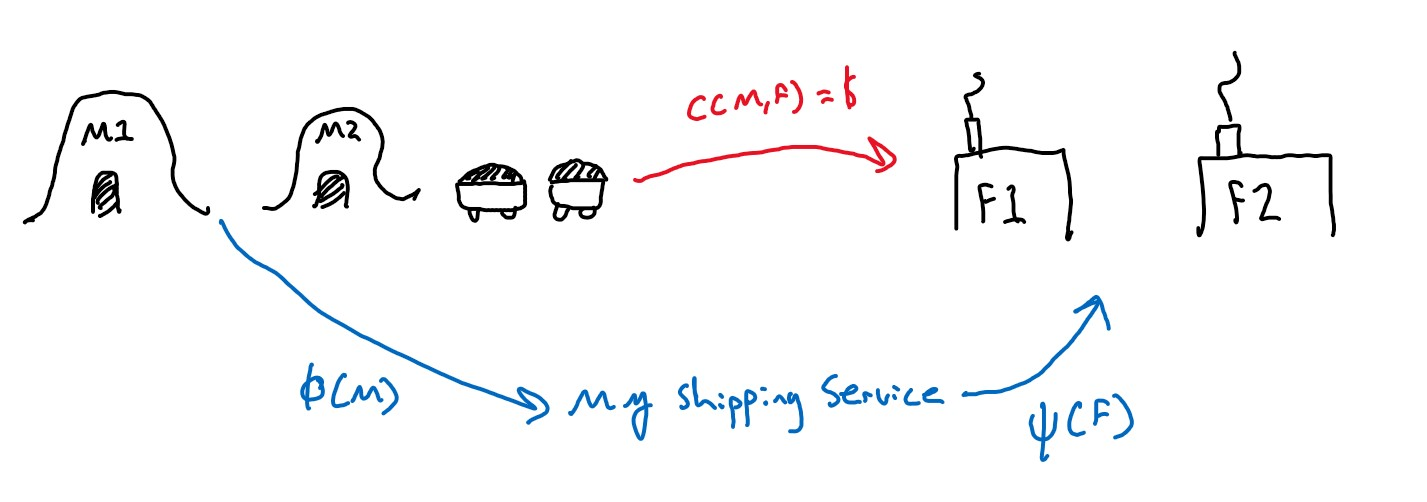
\includegraphics[scale=0.3]{Shippers.jpg}
  \caption{The easiest thing for the owners to do is pay $c(M,F)$, but they can pay less by going through my shipping service which costs $\phi(M) + \psi(F)$.}
\end{figure}
\subsection{Kantorovich Duality}
\begin{thm}[Kantorovich Duality]\label{thm:kant}
Let $X$ and $Y$ be Polish spaces, let $\mu\in \mathcal{P}(X)$ and $\nu\in\mathcal{P}(Y)$, and let\hfill\break $c: X\otimes Y\to \mathbb{R}^+\cup\{+\infty\}$ be a lower semicontinuous cost function.
Whenever $\pi \in \mathcal{P}(X\otimes Y)$ and $(\phi,\psi)\in L^1(d\mu)\otimes L^1(d\nu)$, define 
  \[I(\pi)= \int_{X\otimes Y}c(x,y)d\pi(x,y),\quad J(\phi,\psi) = \int_X\phi d\mu + \int_Y\psi d\nu.\]
  Define $\Pi(\mu,\nu)$ to be the set of all Borel probability measures $\pi$ on $X\otimes Y$ such that for all measurable subsets $A\subset X$ and $B\subset Y$,
  \[\pi(A\otimes Y) = \mu(A),\quad \pi(X\otimes B)= \nu(B),\]
  and define $\Phi_c$ to be the set of all measurable functions $(\phi,\psi)$ satisfying
  \begin{equation}\label{eqn:dualconst}
    \phi(x) + \psi(y) \le c(x,y)
  \end{equation}
  for $d\mu-$almost every $x\in X$, $d\nu-$almost every $y\in Y$. Then,
  \begin{equation}
    \inf_{\Pi(\mu,\nu)} I(\pi) = \sup_{\Phi_c}{J(\phi,\psi)}.
  \end{equation}
\end{thm}
We can construct a minimax principle in order to give an informal proof of \autoref{thm:kant}. We see 
\begin{equation}\label{eqn:minimax}
  \inf_{\pi\in\Pi(\mu,\nu)} \int_{X\times Y}c(x,y)d\pi = \inf_{\pi\in M_+(X\times Y)} \left\{I(\pi)+ \left\{\begin{matrix}0 &\pi\in\Pi(\mu,\nu) \\ +\infty &\text{otherwise.}\end{matrix}\right\} \right\}
\end{equation}
where $M_+$ is the set of nonnegative Borel measures on $X\times Y$. We can rewrite the righthand side of \autoref{eqn:minimax} with
\[\left\{\begin{matrix}0 &\pi\in\Pi(\mu,\nu) \\ +\infty &\text{otherwise.}\end{matrix}\right\} =\sup_{(\phi,\psi)\in L^1(d\mu)\otimes L^1(d\nu)}\left\{J(\phi,\psi)- \int_{X\times Y} [\phi(x)+\psi(y)]d\pi(x,y)\right\}.\]
as $\pi\in \Pi$ follows the constraints defined in \autoref{eqn:const}. Now, the Monge-Kantorovich problem can be written as 
\begin{equation}
  \inf_{\pi\in M_+(X\times Y)}\sup_{(\phi,\psi)}\left\{I(\pi)+\left\{J(\phi,\psi)- \int_{X\times Y} [\phi(x)+\psi(y)]d\pi(x,y)\right\}\right\}.
\end{equation}
Informally exchanging the $\inf$ and $\sup$, we get that the Monge-Kantorovich problem is 
\begin{equation}\label{eqn:swap}
  \sup_{(\phi,\psi)}\inf_{\pi\in M_+(X\times Y)}\left\{I(\pi) - \int_{X\times Y}[\phi(x) +\psi(y)]d\pi(x,y)+J(\phi,\psi)\right\}.
\end{equation}
Now, note that 
\[ \inf_{\pi\in M_+(X\times Y)}\left\{I(\pi) - \int_{X\times Y}[\phi(x) + \psi(y)]d\pi(x,y)\right\} = \left\{\begin{matrix}0 &\phi(x) + \psi(y) \le c(x,y) \\ -\infty &\text{otherwise.}\end{matrix}\right\}\]
so the Kantorovich-Monge problem becomes the maximization (dual) problem
\begin{equation}
  \mathbb{K}(\mu,\nu) = \sup_{\Phi_c}\left\{J(\phi,\psi)\right\}.
\end{equation}
We've assumed that $(\phi,\psi) \in Cb(X)\times C_b(Y)$ as $\phi(x)+\psi(y) \le c(x,y)$ holding everywhere is different to holding almost everywhere. Moreover, we need to make this minimax principle rigorous.
\subsection{Fenchel-Rockafellar and Convex Analysis Results}
In order to prove \autoref{thm:kant}, we need a rigorous minimax principle. We start by presenting some results and definitions from convex and functional analysis.
\begin{defn}[Legendre-Fenchel Transform]
  Let $\phi: E \to \R\cup \{+\infty\}$ be convex. Then, the Legendre-Fenchel Transform for $f\in E^\star$ is
  \begin{equation}
    \phi^\star(f) = \sup_{x\in E}\left[\langle f, x\rangle - \phi(x)\right].
  \end{equation}  
\end{defn}
\begin{defn}[Polish Spaces]
A Polish space, $X$, satisfies the following 
\begin{enumerate}
  \item A Borel probability measure $\mu$ on $X$ is regular
  \item A probability measure $\mu$ on $X$ is concentrated on a $\sigma$-compact set.
  \item Any tight family of probability measures in $\mathcal{P}(X)$ is relatively sequentially compact in $\mathcal{P}(X)$.
  \item Let $X$ be a metric space. If $F$ a nonnegative lower semi-continuous function on $X$ then it can be written as the supremum of an increasing sequence of uniformly continuous nonnegative functions.
  \item If $K$ is a compact metric space then $C(K)$ is separable.
\end{enumerate}
Details of these are presented in \cite{villani} and \cite{billingsey}.
\end{defn}
Now, we introduce the following from \cite{brezis}
\begin{thm}[Fenchel-Rockafellar]\label{thm:Fenchel}
  Let $E$ be a normed vector space and $E^\star$ be its topological dual space. Let $\phi,\psi:E\to\R\cup\{+\infty\}$ be convex. If there is some $x_0\in E$ such that $\phi(x_0),\psi(x_0) <+\infty$ and $\phi$ is continuous at $x_0$, then
  \begin{align*}
    \inf_{x\in E}\{\phi(x)+\psi(x)\} = \max_{f\in E^\star}\{-\phi^\star(-f)-\psi^\star(f)\}.
  \end{align*}
\end{thm}
\begin{proof}
  To be proven. I can base this off of Brezis.
\end{proof}
Moreover, we can check that \autoref{thm:Fenchel} is a minimax principle.
\subsection{Proof of Kantorovich Duality}
Finally, we can begin to prove Kantorovich Duality as stated in \autoref{thm:kant}. The following lemmas come from \cite{villani}.
\begin{lem}\label{lem:kant1}
  Under the same conditions as \autoref{thm:kant}, 
  \begin{equation}\label{eqn:leftineq}\sup_{\Phi_C} J(\phi,\psi) \le \inf_{\Pi(\mu,\nu)} I(\pi).\end{equation}
\end{lem}
\begin{proof}
  Let $(\phi,\psi) \in \Phi_c$ and $\pi\in \Pi(\mu,\nu)$. Then,
  \[J(\phi,\psi) = \int_X\phi d\mu + \int_Y\psi d\nu = \int_{X\times Y}[\phi(x)+\psi(y)]d\pi(x,y)\]
  as $\pi$ has marginals $\mu,\nu$.\newline
  Let $N_x,N_y$ be null sets of $\mu$ and $\nu$ respectively. Because \autoref{eqn:dualconst} holds almost everywhere, \autoref{eqn:dualconst} holds for 
  $(x,y)\in N_x^c \times N_y^c$. Moreover, $\pi(N_x\times Y) = \mu(N_x) = 0$ and $\pi(X\times N_y) = \nu(N_y) = 0$ so $\pi((N_x^c\times N_y^c)^c) = 0$ so \autoref{eqn:dualconst} holds for $\pi$. Thus,
  \begin{equation}
    \int_{X\times Y}[\phi(x)+\psi(y)]d\pi(x,y) \le \int_{X\times Y}c(x,y)d\pi(x,y).
  \end{equation}
  \autoref{eqn:leftineq} is recovered upon taking the supremum on the left-hand side and the infimum on the right-hand side.
\end{proof}
\begin{lem}\label{lem:kant2}
  Under the same conditions as \autoref{thm:kant}, we have 
  \[\sup_{\Phi_c} J(\phi,\psi) \ge \inf_{\Pi(\mu,\nu)} I(\pi)\]
\end{lem}
\cite{villani} presents the proof in 3 steps of increasing generality:
  \begin{enumerate}[1.]
    \item Assuming $X,Y$ are compact and $c(x,y)$ are continuous.
    \item Keeping the assumption that $c(x,y)$ is continuous, but relaxing compactness of $X,Y$.
    \item Only assuming that $c(x,y)$ is lower semi-continuous.
  \end{enumerate}
  Only 1. will use the minimax principle discussed with \autoref{thm:Fenchel} so the proof will be provided below.
\begin{proof}[Proof of 1.]
  Let $E = C_b(X\times Y)$ with norm $\|\cdot\|_\infty$. By Riesz Representation Theorem, its topological dual can be represented by 
  $E^\star = M(X\times Y)$, where $M$ is the space of Borel measures with norm $\|\cdot\|_{TV}$ (total variation norm). Using $\phi,\psi\in L^1$, we introduce 
  \begin{align}
    \Theta &: u\in C_b(X\times Y)\to \begin{cases}
      0 &\text{if } u(x,y)\ge -c(x,y) \\
      +\infty &\text{otherwise,}
    \end{cases} \\
    \Xi &: u\in C_b(X\times Y)\to \begin{cases}
      \int_X \phi d\mu + \int_Y \psi d\nu &\text{if }u(x,y) = \phi(x) + \psi(y)\\
      +\infty&\text{otherwise.}
    \end{cases}
  \end{align}
$\Xi$ is not unique, but still well defined. If $\phi(x) + \psi(y) = \tilde{\phi}(x) + \tilde{\psi}(y)$, then for $s\in\R$, $\phi = \tilde{\phi} + s$ and $\psi = \tilde{\psi} -s$ so \[ \int_X \phi(x)d\mu + \int_Y \psi(y)d\nu = \int_X \tilde{\phi} d\mu + s\left(\int_Xd\mu - \int_Yd\nu\right) + \int_Y\tilde{\psi}d\nu = \int_X \tilde{\phi} d\mu + \int_Y\tilde{\psi}d\nu.\]
Hence $\Xi$ is well defined.\newline
To show that $\Theta$ is convex, let $u,v\in C_b(X\times Y)$ and $\Theta(u),\Theta(v) < +\infty$ so $u(x,y) \ge -c(x,y)$ and $v(x,y) \ge -c(x,y)$. For $t\in [0,1]$, 
\(tu + (1-t)v \ge c.\) It follows that 
\[\Theta(tu + (1-t)v) = 0 = t\Theta(u) + (1-t)\Theta(v).\]
If $\Theta(u) = +\infty$ or $\Theta(v) = +\infty$, then 
\[\Theta(tu + (1-t)v) \le t\Theta(u) + (1-t)\Theta(v).\]
Hence $\Theta$ is convex.\newline
To show that $\Xi$ is convex, let $u(x,y) = \phi_1(x) + \psi_1(y)$ and $v(x,y) = \phi_2(x) + \psi_2(y)$. Now, it follows that 
\[tu + (1-t)v = t\phi_1 + (1-t)\phi_2 + t\psi_1 + (1-t)\psi_2\]
so therefore
\[\Xi(tu + (1-t)v) = \int_{X}t\phi_1 + (1-t)\phi_2d\mu + \int_{Y}t\psi_1 + (1-t)\psi_2d\nu = t\Xi(u) + (1-t)\Xi(v).\]
Now, if $\Xi(u) = +\infty$ or $\Xi(v) = +\infty$, then clearly 
\[\Xi(tu + (1-t)v) \le t\Xi(u) + (1-t)\Xi(v).\]
Hence $\Xi$ is convex.\newline
Now, if we let $u_0\equiv 1$, we have that $\Theta(u_0),\Xi(u_0) < +\infty$ and $\Theta$ continuous at $u_0$ because $c(x,y)$ is nonnegative. 
From here, the assumptions of \autoref{thm:Fenchel} are satisfied so 
\begin{equation}\label{eqn:fenchel}
  \inf_{u\in E}[\Theta(u) + \Xi(u)] = \max_{\pi \in E^\star}[-\Theta^\star(-\pi) - \Xi^\star(\pi)].
\end{equation}
Now computing the righthand side of \autoref{eqn:fenchel}, we see that 
\[\Theta^\star(-\pi) = \sup_{u\in E}\left(-\int_{X\times Y}ud\pi - \Theta(u)\right) = \sup_{u \ge -c} -\int_{X\times Y}ud\pi = \sup_{u\le c}\int_{X\times Y}ud\pi\]
so \[\Theta^\star(-\pi) = \begin{cases}
  \int_{X\times Y} c(x,y)d\pi &\text{if } \pi\in M_+(X\times Y) \\
  +\infty &\text{otherwise.}
\end{cases}\]
where $M_+(X\times Y) \subset M(X\times Y)$ are the positive Borel measures. For $\Xi$, we see that 
\begin{align*}
  \Xi^\star(\pi) &= \sup_{u\in E}\left(\int_{X\times Y}ud\pi - \Xi(u)\right)\\
  & = \sup_{u(x,y) = \phi(x) + \psi(y)}\left(\int_{X\times Y}ud\pi - \int_X\phi(x)d\mu - \int_Y\psi(y)d\nu\right) \\
  &= \sup_{u(x,y) = \phi(x) + \psi(y)}\left(\int_{X\times Y}[\phi(x) + \psi(y)]d\pi - \int_X\phi(x)d\mu - \int_Y\psi(y)d\nu\right)
\end{align*}
We have that 
\[\Xi^\star(\pi) = \begin{cases}
  0 &\text{if }\pi\in\Pi(\mu,\nu) \\
  +\infty &\text{otherwise.}
\end{cases}\]
as the last equality means that $\pi$ has marginals $\mu$ and $\nu$.
Hence the righthand side of \autoref{eqn:fenchel} can be written as 
\begin{equation}\label{eqn:rhs}
  \max_{\pi\in E^\star}[-\Theta^\star(-\pi) - \Xi^\star] = -\min_{\pi\in \Pi(\mu,\nu)} \int_{X\times Y} c(x,y)d\pi = - \inf_{\Pi(\mu,\nu)}I(\pi).
\end{equation}
Now, to consider the lefthand side of \autoref{eqn:fenchel}, we see that, as $C_b\subset L^1$,
\begin{equation}\label{eqn:lhs}
  \inf_{u\in E} [\Theta(u) + \Xi(u)] \ge \inf_{\substack{\phi(x) + \psi(y) \ge -c(x,y)\\ \phi\in L^1(d\mu),\psi\in L^1(d\nu)}} \int_X\phi(x)d\mu + \int_Y\psi(y)d\nu = -\sup_{\Phi_c} J(\phi,\psi).
\end{equation}
Combining \autoref{eqn:rhs} and \autoref{eqn:lhs}, we see that 
\begin{equation}
  - \sup_{\Phi_c}J(\phi,\psi)\le - \inf_{\Pi(\mu,\nu)}I(\pi) \implies \sup_{\Phi_c}J(\phi,\psi)\ge \inf_{\Pi(\mu,\nu)}I(\pi).
\end{equation}
\end{proof}
\begin{proof}[Proof of \autoref{thm:kant}]
  \begin{align*}
    \sup_{\Phi_c}J(\phi,\psi)\le \inf_{\Pi(\mu,\nu)}I(\pi) &\,\,\text{by \autoref{lem:kant1}}. \\
    \sup_{\Phi_c}J(\phi,\psi)\ge \inf_{\Pi(\mu,\nu)}I(\pi) &\,\,\text{by \autoref{lem:kant2}}.
  \end{align*}
  Hence
  \[ \sup_{\Phi_c}J(\phi,\psi)= \inf_{\Pi(\mu,\nu)}I(\pi).\]
\end{proof}
\section{Existence and Characterization of Transport Maps}
Now that we've discussed the Monge-Kantorovich problem and its dual, it's best to describe conditions in which there is existence of optimal transport maps. Transport maps are difficult to characterize 
so we will be restricting to quadratic costs $c(x,y)=|x-y|^2$. There are generalizations that exist, but with additional burden \cite{thorpe}. Moreover, the second assumption we will make is that $X,Y\subset \R^n$. 
\subsection{Characterization of Transport Maps}

The following is theorem 2.12 in \cite{villani}.
\begin{thm}[Brenier's theorem]\label{thm:brenier}
Let $\mu,\nu$ be probability measures on $\R^n$ such that $\int |x|^2 d\mu + \int |y|^2d\nu < +\infty$. If $\mu$ does not give mass to small sets, then there is a unique $\pi\in\Pi(\mu,\nu)$ such that 
\[\pi = (\text{Id}\times \nabla \phi)_\#\mu\]
where $\phi$ is the unique convex function with $\nabla\phi_\#\mu = \nu$.
\end{thm}
\begin{cor}\label{cor:transport}
  Under the same assumptions as \autoref{thm:brenier}, $\nabla\phi$ is the unique solution to the Monge transportation problem:
  \[\int_X|x-\nabla\phi(x)|^2d\mu(x) = \inf_{T\in\mathcal{T}(\mu,\nu)}\int_X|x-T(x)|^2d\mu(x).\]
\end{cor}
\subsection{Optimality and Convex Analysis}
First introducing a few definitions in convex analysis.
\begin{defn}[Convex Conjugate]
  The convex conjugate of a proper function $\phi: \R^n\to\R\cup\{+\infty\}$ is defined by 
  \[\phi^\star = \sup_{x\in\R^n}(x\cdot y - \phi(x)).\]
\end{defn}
\begin{defn}[Subdifferential]
  The subdifferential $\partial \phi$ of a convex function is defined by 
  \[\partial \phi(x) = \{y : \phi(z)\ge \phi(x) + y\cdot(z-x)\text{ for all $z\in \R^n$}\}.\]
\end{defn}
We can now characterize the subdifferential.
\begin{prop}
  Let $\phi$ be a proper, 
\end{prop}
Prior to proving \autoref{thm:brenier}, there are some steps required beforehand. The first of which is the Knott-Smith optimality criterion.
\begin{thm}[Knott-Smith Optimality Criterion]
  Let $\mu,\nu$ be under the same assumptions as \autoref{thm:brenier}. There exists a minimizer $\pi^\dagger\in\Pi(\mu,\nu)$ to the Kantorovich optimal transport problem with cost $c(x,y) = |x-y|^2$ if and only if there exists 
  an $L^1(\mu)$, convex lower semi-continuous function $\phi$ such that $\text{supp}(\pi^\dagger)\subseteq \text{Gra}(\partial \phi)$. Moreover, 
  the pair $(\phi,\phi^\star)$ is a minimizer to the dual problem where $\phi_c$ is defined as 
  \begin{align*}
    \Phi_c = \left\{(\phi,\psi) \in L^1(\mu)\times L^1(\nu) : \phi(x)+\psi(y) \ge x\cdot y\right\}.
  \end{align*}
\end{thm}
\section{Wasserstein}
Metrics such as $L^p$ form a metric based on pointwise differences. We see this when considering the functions $f(x)=\chi_{[0,1]}(x)$ and $f_\delta(x) = \chi_{[\delta,\delta+1]}$, where $\chi_\Omega$ is the indicator function of $\Omega$.
In particular, we see that 
\[\|f-f_\delta\|_{L^p}^p = \begin{cases} 2\delta &\text{if $|\delta| < 1$} \\
2 &\text{otherwise.}\end{cases}\]
We see that when $|\delta| \ge 1$, the sets $[0,1]$ and $[\delta,\delta+1]$ are disjoint and the $L^p$ distance is constant. This is potentially a problem because if $\delta$ is set large, $\frac{d}{d\delta}\|f_\delta - f \|_{L^p} = 0$, which is a problem in gradient based optimization.\newline
Rather, if we look for a optimal transport cost using $f$ and $f_\delta$, we have the following problem 
\[\min_{T_\#f = f_\delta}\ \int_0^1|x-T(x)|^pdx = |\delta|^p\]
where $f$ and $f_\delta$ are defined as the measures with density $f$ and $f_\delta$ respectively. This example comes from \cite{thorpe}.\newline
Moreover, if we let $f,g$ be functions in $\R^n$, we can intuitively describe $L^p$ as the vertical distance between functions $f$ and $g$ while the optimal transport problem with cost $d(x,y)^p$ can be seen as the horizontal distance between measures with density $f$ and $g$. The figure from \cite{santambrogio} is shown below.
\begin{figure}[H]
  \center
  
\includegraphics[scale=0.5]{banner.jpg}
  \caption{The "vertical" and "horizontal" differences described between the $L^p$ cost and the optimal transport cost. $T(x)$ is the optimal transport cost, not to be confused with the optimal transport map.}
\end{figure}
\subsection{Wasserstein Distances}
Let's start by considering Kantorovich-Monge solutions to the transport problem with cost functions $c(x,y) = d(x,y)^p$ where $d$ is the distance on $X$ and $Y$.
Let $\Omega\subset X$ and set $x_0\in X$.
\[\mathcal{P}_p(X) = \left\{\mu\in\mathcal{P}(X):\int_{\Omega}d(x,x_0)^p < +\infty\right\}\]
is the admissable class of measures $\mu$, even if $X$ is unbounded.
\begin{lem}[Kantorovich-Monge forms a metric.]\label{lem:wass}
	Let \[W_p(\mu,\nu) = \left[\inf_{\pi\in\Pi(\mu,\nu)}\int_{X\times X}d(x,y)^pd\pi(x,y)\right]^{1/p}\] defined for $\mu,\nu\in\mathcal{P}_P(X)$ be the Wasserstein Distance. This forms a metric on $X$.
\end{lem}
\begin{proof}
  \begin{enumerate}
    \item Because $d(x,y) \ge 0$, it's clear that $W_p$ is nonnegative. 
    \item The product measure $\mu\times \nu = \nu\times \mu$, so $W_p$ is symmetric.
    \item[*] It's sufficient to show for (1), (2) that $W_p$ is finite on $P_p$. For any $\Omega\subset X$,
    \begin{equation}W_p(\mu,\nu) \le p \inf_{\pi\in\Pi(\mu,\nu)}\int_{\Omega\times \Omega} |x|^p + |y|^pd\pi(x,y) = p\int_\Omega|x|^pd\mu(x) + p\int_{\Omega}|y|^pd\nu(y).\end{equation}
    This is finite because $\mu,\nu\in \mathcal{P}_p(\Omega)$.
    \item  $W_p(\mu,\mu) = 0$ as $d(x,T(x)) = 0$ if $T_\# \mu = \mu$. Conversely, let $\mu,\nu\in \mathcal{P}_p(X)$ such that $W_p(\mu,\nu) = 0$. Let $\pi$ be an optimal transportation plan. 
    In order for this to be possible, $\pi$ is supported on the diagonal $x=y$. Hence, for all $\phi\in C_b(X)$,
    \[ \int \phi d\mu = \int \phi(x)d\pi(x,y) = \int\phi(y)d\pi(x,y) = \int\phi d\nu\]
    which implies $\mu=\nu$.
    \item   Assume $\mu,\nu,\eta\in \mathcal{P}_p(X)$ are absolutely continuous. Let $T$ be the optimal map from $\mu$ to $\eta$ and $S$ be the optimal map from $\eta$ to $\nu$.
    Then $S\circ T\in \mathcal{T}(\mu,\nu)$ because $(S\circ T)_\#\mu = S_\#(T_\#\mu) = S_\#\eta = \nu$. Hence,
    \begin{align*}
      W_p(\mu,\nu)) &\le \left(\int_Xd(x,(S\circ T)(x))^pd\mu(x)\right)^{1/p} = \|d(\text{Id},(S\circ T))\|_{L^p(\mu)} \\
      &\le \|d(\text{Id},T)\|_{L^p(\mu)} + \|d(T, S\circ T)\|_{L^p(\mu)} \\
      &= W_p(\mu,\eta) + \|d(\text{Id}, S)\|_{L^p(\eta)} \\
      &= W_p(\mu,\eta) + \int_{X}d(x,S(x))^pd\eta(x) = W_p(\mu,\eta) + W_p(\eta,\nu).
      \end{align*}
  \end{enumerate}
\end{proof}
The proof of the triangle inequality above takes a further assumption that $\mu$ and $\nu$ are absolutely continuous with respect to the Lebesgue measure.
Moreover, the proof regarding a gluing lemma is found in the proof of theorem 7.3 in \cite{villani}.
\begin{prop}[Ordering of Wasserstein]
  For every $p\in [1,+\infty)$, and any $\mu,\nu\in \mathcal{P}_p(X)$, we have that $W_p(\mu,\nu) \ge W_1(\mu,\nu)$. Furthermore, if $X$ is bounded, then $W_p(\mu,\nu)^p \le \text{diam}(X)^{p-1}W_1(\mu,\nu)$.
\end{prop}
\begin{proof}
  By Jensen's inequality,
  \begin{equation*}
    \left(\int_{X\times X} d(x,y)^pd\pi(x,y)\right)^{1/p} \ge \int_{X\times X} d(x,y)d\pi(x,y)
  \end{equation*}
  Hence, $W_p(\mu,\nu) \ge W_1(\mu,\nu)$ as this holds for all $\pi\in \Pi(\mu,\nu)$.\newline
  Now if $X$ is bounded, then for all $x,y\in X$,
  \begin{align*}
    d(x,y)^p \le (\max_{w,z\in X} d(w,z)^{p-1})d(x,y) = \text{diam}(X)^{p-1}d(x,y). \\
    \int_{X\times X} d(x,y)d\pi(x,y)\le (\text{diam}(X)^{p-1})\int_{X\times X}d(x,y)d\pi(x,y).
  \end{align*}
  It follows $W_p(\mu,\nu) \le \text{diam}(X)^{p-1}W_1(\mu,\nu).$
\end{proof}
\subsection{Wasserstein Topology}
We see that if $x_n\to x$ in $X$ then
\(W_p(\delta_{x_n},\delta_x) = d(x_n,x)^{\inf{(1,p)}} \to 0\). Furthermore, another hint to the topology induced by the Wasserstein distance is the fact that it's not very sensitive to oscillation.
\begin{exmp}
  For $k\ge 1$, consider $f_k(x)=1+\sin(2\pi k x)$ on the line segment $[0,1]$. Let $du_k(x) = f_k(x)dx$ and let $\mathcal{L}$ be the Lebesgue measure on $[0,1]$. Let $p\ge 1$ and show that $W_p(\mu_k,\mathcal{L}) \le C_pk^{-1}$ for some constant $C_p$ depending only on $p$.
\end{exmp}
\begin{proof}
  $W_p(\mu_k,\mathcal{L}) \le \int_{[0,1]\times[0,1]}(1+\sin{2\pi k x})|x-y|^pdxdy$
\end{proof}
The following theorem is from \cite{villani}.
\begin{thm}[Wasserstein distances metrize weak convergence]\label{thm:weak}
	Let $p\in(0,\infty)$, let $(\mu_k)_{k=1}^\infty$ be a sequence of measures in $\mathcal{P}_p(X)$ and $\mu\in \mathcal{P}(X)$, then the following are equivalent
  	\begin{enumerate}[(i)]
		\item $W_p(\mu_k,\mu)\to 0$
		\item $\mu_k\to\mu$ in the weak sense, and for any $x_0\in X$, 
		\[\lim_{R\to\infty}\limsup_{k\to\infty} \int_{d(x_0,x)\ge R} d(x_0,x)^pd\mu_k(x) = 0.\]
    \item $\mu_k\to\mu$ in the weak sense, and for any $x_0\in X$, 
    \[\int d(x_0,x)^pd\mu_k(x) \to \int d(x_0,x)^pd\mu < +\infty.\]
    \item Whenever a continuous function $\phi$ on $X$ satisfies the growth condition $|\phi(x)| \le C(1+d(x_0,x)^p)$ for some $x_0\in X$ with $C\in \R$, then $\int |\phi(x)|d\mu(x) < +\infty$ and 
     \[\int \phi d\mu_k \to \int \phi d\mu.\]
	\end{enumerate} 
\end{thm}
\begin{proof}[proof from \cite{villani}]
  Without loss of generality, let $p\ge 1$ and the assumptions of \autoref{thm:weak} be satisfied.
  \begin{enumerate}
    \item[$(iv)$] $\implies (iii)$. We see that for any $x_0\in X$, $d(x_0,x)^p \le 1+d(x_0,x)^p$ and $d$ is continuous so $(iii)$ follows from $(iv)$ because $|d| = d$.
    \item[$(ii)$] $\implies (iv)$. Pick an arbitrary continuous function $\phi$ satisfying the growth condition in $(iv)$. Now write, for any $R > 1$,
    \[\phi = \phi_R + \psi_R\]
    where $\phi_R = \inf(\phi(x), C(1+R^p))$ and $\psi_R = \phi(x) - \phi_R(x)$. We see then that $\psi_R$ is pointwise bounded by $C d(x_0,x)^p\chi_{d(x_0,x) \ge R}$ from the growth condition. Then, 
    \begin{align*}
      \left|\int \phi d\mu_k - \int \phi d\mu\right| \le \left|\phi_Rd(\mu_k - \mu)\right| + C\left|\int_{d(x_0,x) \ge R}d(x_0,x)^p[d\mu_k + d\mu](x)\right|
    \end{align*}
    Then, it follows 
    \begin{align*}
      \limsup_{k\to\infty}\left|\int \phi d\mu_k - \int \phi d\mu\right| \le \limsup_{k\to\infty}C\left|\int_{d(x_0,x) \ge R}d(x_0,x)^p[d\mu_k + d\mu](x)\right|
    \end{align*}
    Then, allowing $R\to\infty$, the righthand side tends to 0 as $d(x_0,x) \ge R \to \emptyset$. This shows that $(ii)\implies (iv)$.
    \item[$(iii)$] $\implies (ii)$. This has an inequality I don't exactly get $\dots$ 
  \end{enumerate}
  All that's required now is to show that $(i)\implies(iii)$. However, let's start with noticing 
  \begin{align*}
    \int d(x_0,x)^pd\mu(x) &= \lim_{R\to\infty}\lim_{k\to\infty} \int\inf(d(x_0,x),R)^pd\mu_k(x) \\
    &\le \liminf_{k\to\infty}\int d(x_0,x)^pd\mu_k(x).
  \end{align*}
  Therefore, convergence of the moment of order $p$ in $(iii)$ is equivalent to 
  \begin{equation}
    \limsup_{k\to\infty}\int d(x_0,x)^pd\mu_k(x)\le \int d(x_0,x)^pd\mu(x).
  \end{equation}
\end{proof}
\subsection{Wasserstein as a Geodesic Space}
\section{Gradient Flows and PDEs}
\subsection{Gradient Flow Motivation}
\subsubsection{Fluid Mechanics}
One of the oldest and most basic equations in fluid mechanics is the Euler equation. 
\begin{defn}[Euler's Equation]
  Let open $\Omega\subset\R^n$ be a bounded and smooth. The incompressible Euler equation has
  \begin{equation}
    \begin{cases}
      v_t + v \cdot \nabla v = - \nabla p. \\
      \nabla \cdot v = 0.
    \end{cases}
  \end{equation}
  where $v(t,x): \R_+ \times \Omega \to \R^n$ is the velocity field of a fluid and $p(t,x):\R_+\times \Omega \to \R^n$ is the pressure of the fluid. Moreover, this must be supplemented with the boundary condition, $v$ is tangent to $\partial \Omega$.
\end{defn}
\subsection{Continuity Equation}
The continuity equation is defined with 
\begin{equation}\label{eqn:continuity}p_t + \nabla \cdot (p\vec{v}) = 0\end{equation}
where $p$ is the fluid density and $\vec{v}$ is the flow vector field.\newline
Now, consider the smooth vector field $\vec{v}: [0,\infty)\times \mathbb{R}^n\to \mathbb{R}^n.$
Let $\phi_t: \mathbb{R}^n\to \mathbb{R}^n$ be the flow map such that for each $x\in \mathbb{R}^n$,
\[\partial_t\phi_t(x) = \vec{v}(t,\phi_t(x)),\quad \phi_0(x) = x.\]
Given some measure $p_0$ on $\mathbb{R}^n$, we can look at the family of measures 
\[p_t := (\phi_t)_\# p_0.\]
\begin{thm}
	The family of measures $p_t$ is the unique distributional solution of the IVP of \eqref{eqn:continuity} with initial data $p_t\vert_{t=0} = p_0$.
\end{thm}
\begin{proof}
	Let $\phi\in C^\infty_c(\mathbb{R}^n)$.
	\begin{align*}
		&\int_0^T \int_{\mathbb{R}^n}\partial_t\phi(t,x) + \vec{v}(t,x)\cdot \nabla\phi(t,x)dp_t(x)dt\\
	  = &\int_0^T\int_{\mathbb{R}^n}\partial_t\phi(t,\Phi_t(x)) + \vec{v}(t,\Phi_t(x))\cdot \nabla\phi(t,\Phi_t(x))dp_0(x)dt \\
	  = &\int_{\mathbb{R}^n}\int_0^T \frac{d}{dt}[\phi(t,\Phi_t(x))]dtdp_0(x) = - \int_{\mathbb{R}^n}\phi(0,x)dp_0(x).
	\end{align*}
	Hence $p_t$ is a distributional solution. Uniqueness follows considering $\mu_t = \phi_t-\nu_t$ where $\nu_t$ is another solution.
\end{proof}
\subsection{Benamou-Brenier Theorem}
Restrict $0\le t \le 1$ and fix source ($p_0$) and destination ($p_1$) densities.
\begin{thm}[Bernamou-Brenier]
	The minimum effort required to transport $p_0$ to $p_1$ by the flow of the vector field $\vec{v}$ with $p_t$,
	\begin{equation}
		\inf\left\{A[p_t,v]\bigg\vert\partial_t p_t + \nabla \cdot (p_t \vec{v}) = 0,p_t\vert_{t=0}=p_0, p_t\vert_{t=1}=p_1\right\}
	\end{equation} 
	is equivalent to the squared $2-$Wasserstein Distance $W_2(p_0,p_1)^2$ where \[A[p_t,v] = \int_0^1\int_{\mathbb{R}^n} |\vec{v}(t,x)|^2p_t(x)dxdt\]
\end{thm}
$A$ is also called the action where the inner integral is the kinetic energy $E$ at time $t$. The action can also be interpreted as the average kinetic energy over $0\le t \le 1$. 
\begin{proof}
	Choose admissable $\vec{v},p_t$. We know that $p_t = (\Phi_t)_\#p_0$ where $\Phi$ is the flow map of $V$.
	\begin{align*}
		\int_{\mathbb{R}^n}|\vec{v}(t,x)|^2p_t(x)dx &= \int_{\mathbb{R}^n}|\vec{v}(t,x)|^2 d(\Phi_t)_\#p_0\\
		&= \int_{\mathbb{R}^n}|\vec{v}(t,\Phi_t(x))|^2p_0(x)dx = \int_{\mathbb{R}^n}|\partial_t\Phi_t(x)|^2p_0dx
	\end{align*}
	Using Fubini's theorem and Jensen's inequality,
	\begin{align*}
		A[p_t,v] &= \int_0^1\int_{\mathbb{R}^n}|\partial_t\Phi_t(x)|^2p_0dxdt= \int_{\mathbb{R}^n}\left(\int_0^1|\vec{v}(t,\Phi_t(x))|^2dt\right)p_0(x)dx \\
		&\ge \int_{\mathbb{R}^n}\left(\int_0^1\partial_t\Phi_t(x)dt\right)^2p_0(x) = \int_{\mathbb{R}^n}|\Phi_1(x) - x|^2p_0(x)dx\\
		& \ge W_2(p_0,p_1)^2.
	\end{align*}
\end{proof}
\begin{thebibliography}{9}
\bibitem{villani}
Villani C.
Topics in Optimal Transportation.
American Mathematical Society, 2003.
\bibitem{thorpe}
Thorpe M.
Introduction to Optimal Transport.
University of Cambridge, 2018.
\bibitem{brezis}
Brezis H.
Functional Analysis, Sobolev Spaces and Partial Differential Equations. 
Springer Press, 2011.
\bibitem{billingsey}
Billingsley P.
Convergence of Probability Measures.
John Wiley \& Sons Inc., 1999.
\bibitem{evans}
Evans C. L.
Partial Differential Equations.
American Mathematical Society, 2010.
\bibitem{santambrogio}
Santambrogio, F.
Optimal Transport for Applied Mathematicians
Springer Press, 2015
\end{thebibliography}


\end{document}

